\documentclass{article}  
% Include all project wide packages here.
\usepackage{fullpage}
\usepackage{polyglossia}
\setmainlanguage{dutch}
\usepackage{csquotes}
\usepackage{graphicx}
\usepackage{epstopdf}
\usepackage{pdfpages}
\usepackage{caption}
\usepackage[list=true]{subcaption}
\usepackage{float}
%\usepackage{mathtools}
\usepackage{standalone}
\usepackage{import}
\usepackage{tocloft}
\usepackage{wrapfig}
\usepackage{authblk}
\usepackage{array}
\usepackage{booktabs}
\usepackage[toc,page,title,titletoc]{appendix}
\usepackage{xunicode}
\usepackage{amsmath}
\usepackage{fontspec}
\usepackage{unicode-math}
\usepackage[
    backend=bibtexu,
	texencoding=utf8,
bibencoding=utf8,
    style=ieee,
    sortlocale=nl_NL,
    language=auto
]{biblatex}
\usepackage{listings}
\newcommand{\includecode}[3][c]{\lstinputlisting[caption=#2, escapechar=, style=#1]{#3}}
\newcommand{\superscript}[1]{\ensuremath{^{\textrm{#1}}}}
\newcommand{\subscript}[1]{\ensuremath{_{\textrm{#1}}}}


\newcommand{\chapternumber}{\thechapter}
\renewcommand{\appendixname}{Bijlage}
\renewcommand{\appendixtocname}{Bijlagen}
\renewcommand{\appendixpagename}{Bijlagen}

\usepackage[hidelinks]{hyperref} %<--------ALTIJD ALS LAATSTE
  
\renewcommand{\familydefault}{\sfdefault}

\setmainfont[Ligatures=TeX]{Myriad Pro}
\setmathfont{Asana Math}
\setmonofont{Lucida Console}

\usepackage{titlesec, blindtext, color}
\definecolor{gray75}{gray}{0.75}
\newcommand{\hsp}{\hspace{20pt}}
\titleformat{\chapter}[hang]{\Huge\bfseries}{\chapternumber\hsp\textcolor{gray75}{|}\hsp}{0pt}{\Huge\bfseries}
\renewcommand{\familydefault}{\sfdefault}
\renewcommand{\arraystretch}{1.2}
\setlength\parindent{0pt}

%For code listings
\definecolor{black}{rgb}{0,0,0}
\definecolor{browntags}{rgb}{0.65,0.1,0.1}
\definecolor{bluestrings}{rgb}{0,0,1}
\definecolor{graycomments}{rgb}{0.4,0.4,0.4}
\definecolor{redkeywords}{rgb}{1,0,0}
\definecolor{bluekeywords}{rgb}{0.13,0.13,0.8}
\definecolor{greencomments}{rgb}{0,0.5,0}
\definecolor{redstrings}{rgb}{0.9,0,0}
\definecolor{purpleidentifiers}{rgb}{0.01,0,0.01}


\lstdefinestyle{csharp}{
language=[Sharp]C,
showspaces=false,
showtabs=false,
breaklines=true,
showstringspaces=false,
breakatwhitespace=true,
escapeinside={(*@}{@*)},
columns=fullflexible,
commentstyle=\color{greencomments},
keywordstyle=\color{bluekeywords}\bfseries,
stringstyle=\color{redstrings},
identifierstyle=\color{purpleidentifiers},
basicstyle=\ttfamily\small}

\lstdefinestyle{c}{
language=C,
showspaces=false,
showtabs=false,
breaklines=true,
showstringspaces=false,
breakatwhitespace=true,
escapeinside={(*@}{@*)},
columns=fullflexible,
commentstyle=\color{greencomments},
keywordstyle=\color{bluekeywords}\bfseries,
stringstyle=\color{bluestrings},
identifierstyle=\color{purpleidentifiers}
}

\lstdefinestyle{vhdl}{
language=VHDL,
showspaces=false,
showtabs=false,
breaklines=true,
showstringspaces=false,
breakatwhitespace=true,
escapeinside={(*@}{@*)},
columns=fullflexible,
commentstyle=\color{greencomments},
keywordstyle=\color{bluekeywords}\bfseries,
stringstyle=\color{redstrings},
identifierstyle=\color{purpleidentifiers}
}

\lstdefinestyle{xaml}{
language=XML,
showspaces=false,
showtabs=false,
breaklines=true,
showstringspaces=false,
breakatwhitespace=true,
escapeinside={(*@}{@*)},
columns=fullflexible,
commentstyle=\color{greencomments},
keywordstyle=\color{redkeywords},
stringstyle=\color{bluestrings},
tagstyle=\color{browntags},
morestring=[b]",
  morecomment=[s]{<?}{?>},
  morekeywords={xmlns,version,typex:AsyncRecords,x:Arguments,x:Boolean,x:Byte,x:Char,x:Class,x:ClassAttributes,x:ClassModifier,x:Code,x:ConnectionId,x:Decimal,x:Double,x:FactoryMethod,x:FieldModifier,x:Int16,x:Int32,x:Int64,x:Key,x:Members,x:Name,x:Object,x:Property,x:Shared,x:Single,x:String,x:Subclass,x:SynchronousMode,x:TimeSpan,x:TypeArguments,x:Uid,x:Uri,x:XData,Grid.Column,Grid.ColumnSpan,Click,ClipToBounds,Content,DropDownOpened,FontSize,Foreground,Header,Height,HorizontalAlignment,HorizontalContentAlignment,IsCancel,IsDefault,IsEnabled,IsSelected,Margin,MinHeight,MinWidth,Padding,SnapsToDevicePixels,Target,TextWrapping,Title,VerticalAlignment,VerticalContentAlignment,Width,WindowStartupLocation,Binding,Mode,OneWay,xmlns:x}
}

%defaults
\lstset{
basicstyle=\ttfamily\small,
extendedchars=false,
numbers=left,
numberstyle=\ttfamily\tiny,
stepnumber=1,
tabsize=4,
numbersep=5pt
}  
\usepackage{graphicx}
\usepackage{hyperref}


\author{
Tu Hoang(4203496) \and Peter Stijnman (4215788) \and Alex Janssen (4231333) \\
}
\title{TU Delft EPO3-1 - Opdracht 4: Process Variaties}
\date{9 Oktober 2013}
\begin{document}
\maketitle

\section{Abstract}

Dit verslag gaat over process variaties tijdens de fabricage van transistoren die ervoor zorgen dat er een andere stroom gaat lopen door de transistor. Met een aantal parameters die kunnen variëren, Vdd, de drempelspanning, de dikte van de oxidelaag, de lengte en de breedte van de transistor, wordt er gesimuleerd en gekeken wat deze variaties tot gevolg hebben op de stroom door de transistor. Als uitkomst hebben we gekregen dat de lengte de grootste rol speelt in het vergroten van de stroom, bij een kleinere lengte komt een een grotere stroom.
Bij de NMOS was de stroom $I_d$ =  0,005997 A variërend van -16% tot + 20%. voor PMOS conden wij een stroom voor $I_d$ = -0,00128  A  variërend van +13% tot -21%. Met negatieve percentages wordt bedoeld dat de stroom verder naar de nul gaat of verder de min in.

\tableofcontents
\clearpage

\section{Inleiding}
Het doel van deze opdracht is om meer kennis op te doen over MOSFET transistoren, in specifiek meer over de variatie in de productie hiervan. Tijdens het produceren van de transistoren zijn er bepaalde foutmarges in bijvoorbeeld de lengte en de breedte van de transistor. In dit verslag gaan we kijken wat deze foutmarges voor een invloed hebben op de uiteindelijke stroom die er door de transistor gaat lopen. In het verloop van de rest van dit project zullen we met deze process variaties rekening moeten houden voor het uiteindelijke ontwerp, het is daarom handig dat we daar nu al aandacht aan besteden.\\
Het verslag bestaat uit een probleemstelling, een theorie die bespreekt waardoor de process variaties onstaan, hoe we deze opdracht hebben aangepakt gevolgt door de simulatie met resultaten en als laatste een discussie over de resultaten en de conclusie om het af te ronden.

\section{Probleemstelling}
\textbf{Process Variaties}\\
In de praktijk zullen de transistoreigenschappen varieren van device tot device, van chip tot chip en van 
wafer tot wafer. Zie Sectie 3.4 van het boek. Bepaal welke combinatie van parameterafwijkingen hieronder
de transistor oplevert met de grootste en met de kleinste maximale stroom (bij maximale VGS en maximale
VDS) en bepaal de waarden van de maximale en minimale stroom.\\
Met als variaties:
\newline
\begin {itemize}
	\item Vdd \pm 10\%
	\item Vt0  \pm 120mV
	\item Tox \pm 5\%
	\item L \pm 0.1\textmu m
	\item W \pm 0.1\textmu m
\end {itemize}

Om deze variaties te kunnen simuleren, is het nodig om de modelparameters (zie de ModelLibEPO3.lib
file) aan te passen. Sommige parameters zijn aan te passen in de schematic editor, voor sommige moet je
misschien de .lib file aanpassen. Geef in het rapport ook kwalitatieve verklaringen van de effecten die je
ziet.

\section{Theorie}

Hoewel in theorie alle transistoren van hetzelfde type als identiek worden beschouwd, is dit natuurlijk in het echt niet het geval. 
Bij elke wafer zullen die parameters van een transistor net iets anders zijn en daar moet dus ook rekening worden gehouden tijdens het ontwerpen van een schakeling. Deze verschillen in de parameters komt voornamelijk door het resultaat van twee factoren:
\newline
\begin {itemize}
	\item Variaties in het process ,zoals dat het materiaal niet overal even zuiver is, de dikte van de oxidelaag, de diffusie dieptes, die komen door in verandering in omstandigheden tijdens het maken van de transistor. Het resultaat hiervan is dat de vierkantsweerstand veranderd, en transistor parameters zoals de drempelspanning.
	\item Variaties in de demensies van het apparaat, als resultaat van de gelimiteerde nauwkeurigheid van het printen. Dit veroorzaakt bijvoorbeeld veranderingen in de W/L verhoudingen en de breedte van verbindende draden.
\end {itemize}

Gelukkig komen de beste en slechste gevallen qua variaties niet vaak voor. Meestal zijn de waardes van de variatie normaal verdeeld. 
Tijdens het ontwerpen van een schakeling moet dus een afweging gemaakt worden tussen betrouwbaarheid van de schakeling en de complexiteit van de schakeling, er wordt vaak voor gekozen om rond een 98\% betrouwbaarheid van de schakeling te zitten. Dit wil dus zeggen dat 98\% van alle geproduceerde schakelingen het doen zoals in de specificaties gemeld wordt. Als je een hoger percentage wilt hebben dan wordt automatisch je schakeling ook groter en complexer en dat is het vaak niet waard.\\
Al deze variaties zorgen ervoor dat er een andere stroom door de transistor gaat lopen. En zo kan het dus zijn dat er fouten optreden in de logica van de schakeling.[1] De stroom de transistor wordt gegeven door[2],
\newline
\begin {equation}
	I_D = \textmu _{n}\varepsilon _{ox}/t_{ox}W/L(V_{GT}*V_{MIN} - 0.5V_{MIN}^2)(1+\lambda V_{DS})    \mathrm{~~~voor~~~}    V_{GT}>= 0
\end {equation}
 met 
\begin {equation}
	V_{MIN} = MIN(V_{DS},V_{GT},V_{DSAT})
\end {equation}

De minimale stroom wordt bepaald door de volgende waardes van de  parameters te minimaliseren of te maximaliseren.
\begin{itemize}
	\item minimaliseer Vdd ,de breedte
	\item maximaliseer tox, Vto, de lengte
\end{itemize}

Voor de maximale waarde van de stroom moet dit natuurlijk precies andersom.

\begin{itemize}
	\item maximaliseer Vdd ,de breedte
	\item  minimaliseer tox, Vto, de lengte
\end{itemize}


\section{Aanpak}

Om te kijken wat al deze variaties voor een invloed hebben gaan we eerst voor alle parameters apart kijken hoe de stroom door de transistor gaat veranderen. We willen dit zo duidelijk mogelijk in beeld brengen dus hebben voor elke parameter de maximale afwijking genomen om mee te simuleren. En als laatste kijken we wat de grootste en de kleinste stroom door de transistor kan zijn door deze afwijkingen.Als referentie transistor nemen we een perfect gemaakte transistor, dit betekent een transistor zonder afwijkingen.\\
Het simuleren gaat met het programma PSpice en vanuit daar exporteren we de data naar een Excel sheet. Hier kunnen we duidelijk mooie leesbare grafieken maken en blijft alle data in de sheet zelf ook overzichtelijk.

\clearpage

\section{De Simulatie}
 
In PSpice hebben we een simpel circuit gesimuleerd met alleen maar de transistor en de bronnen om hem aan te sturen. Het circuit zag er als volgt uit,

\begin{figure}[H]
	\centering
	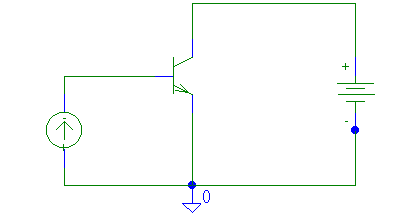
\includegraphics[width=0.5\textwidth]{transistorsim}
	\caption {Transistor circuit}
\end{figure}

Verder hebben we bij het simuleren een transient analysis gedaan zodat we voor een groter bereik van Vdd konden zien wat er met de stroom gebeurde.
Tijdens het simuleren moesten we de parameters van de transistor veranderen in de library file zodat PSpice met de juiste variaties werkte en zo hebben we het effect van alle parameters apart onderzocht en hebben we gekeken wat de maximale en de minimale stroom zou opleveren.Bij het veranderen van de parameters apart hielden we de rest van de waardes op de standaard ingestelde waardes van de library.

\clearpage

\section{Resultaten}

In elk van de volgende grafieken zijn de standaard waardes van de transistor weergegeven en van de parameter die we onderzochten de minimale en maximale afwijking.
Als eerste hebben we gesimuleerd voor de drempelspanning (Vto).

\begin{figure}[H]
	\centering
	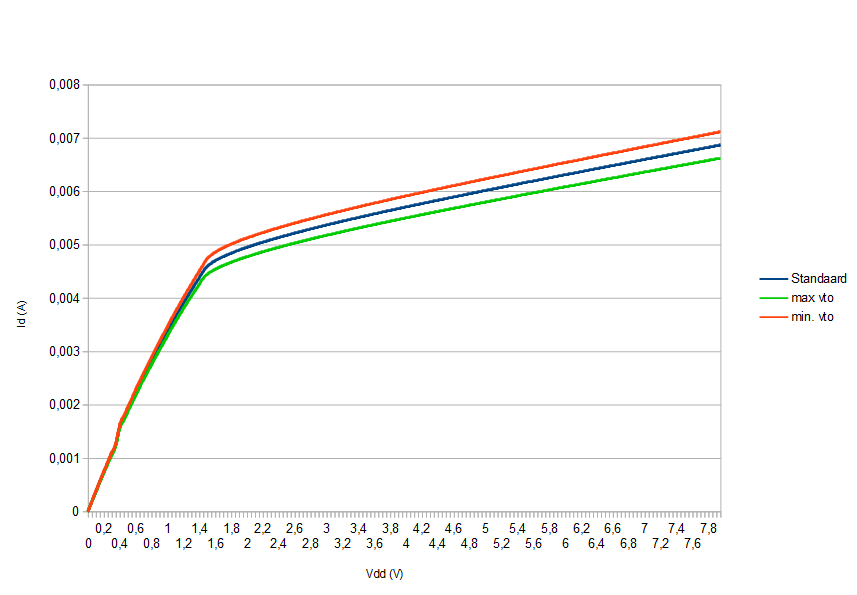
\includegraphics[width=0.7\textwidth]{nmosvto}
	\caption{NMOS met Vto als parameter}
\end{figure}

\begin{figure}[H]
	\centering
	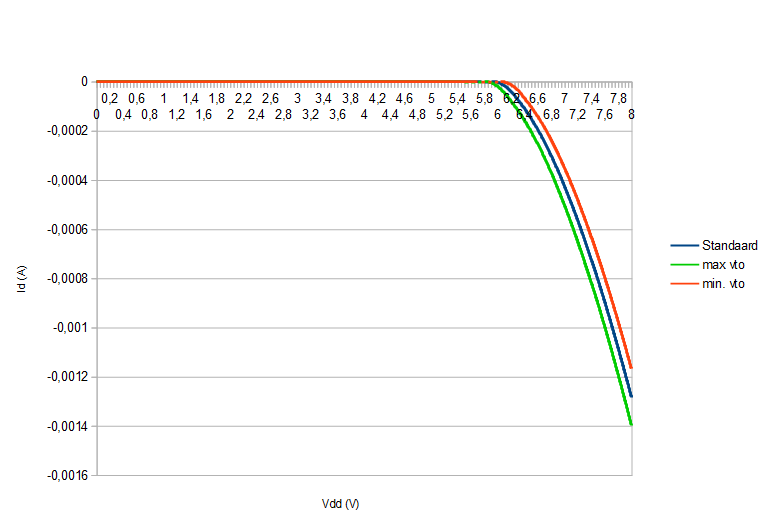
\includegraphics[width=0.7\textwidth]{pmosvto}
	\caption{PMOS met Vto als parameter}
\end{figure}
\clearpage

Hierna hebben het effect van de dikte van de oxidelaag gesimuleerd(tox).

\begin{figure}[H]
	\centering
	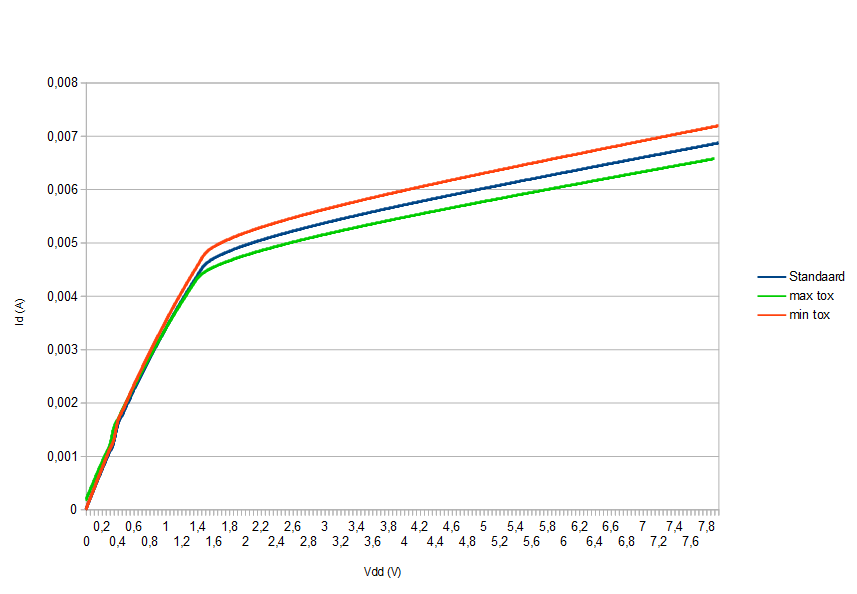
\includegraphics[width=0.8\textwidth]{nmostox}
	\caption{NMOS met tox als parameter}
\end{figure}

\begin{figure}[H]
	\centering
	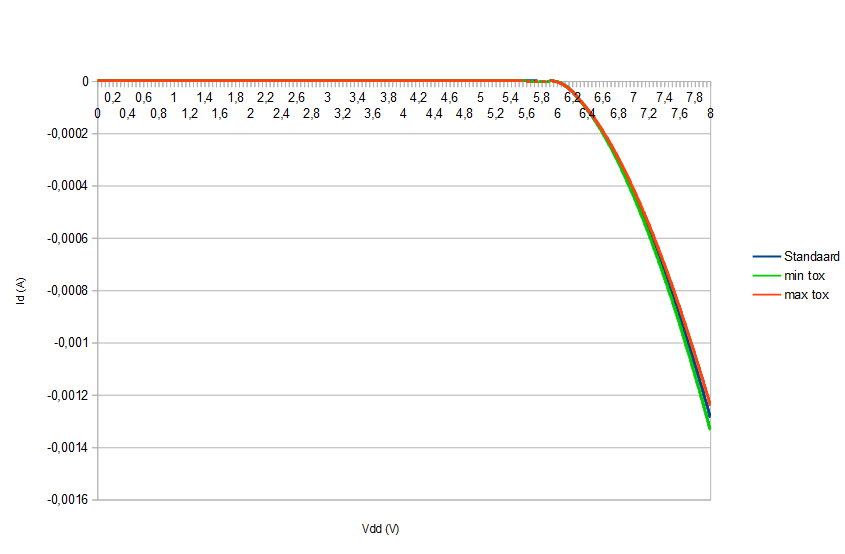
\includegraphics[width=0.8\textwidth]{pmostox}
	\caption{PMOS met tox als parameter}
\end{figure}

\clearpage
Als derde op het lijstje stond de lengte van de condensator(L)

\begin{figure}[H]
	\centering
	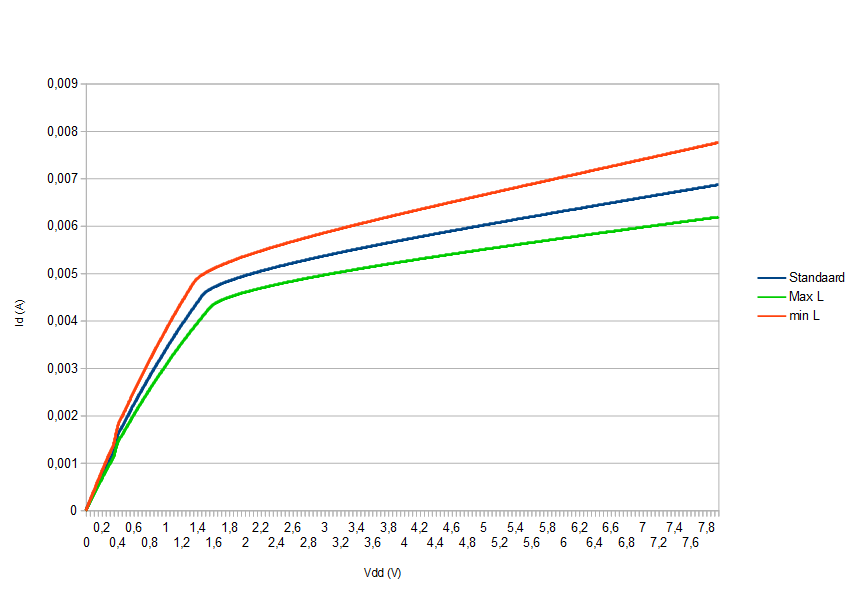
\includegraphics[width=0.8\textwidth]{nmoslengte}
	\caption{NMOS met de lengte als parameter}
\end{figure}

\begin{figure}[H]
	\centering
	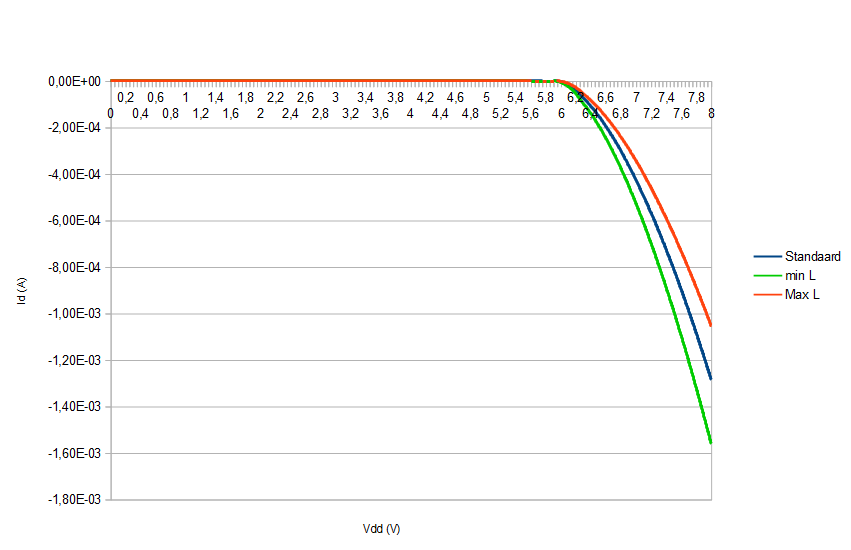
\includegraphics[width=0.8\textwidth]{pmoslengte}
	\caption{PMOS met de lengte als parameter}
\end{figure}

\clearpage
Hierna volgde natuurlijk de breedte van de transistor(W).

\begin{figure}[H]
	\centering
	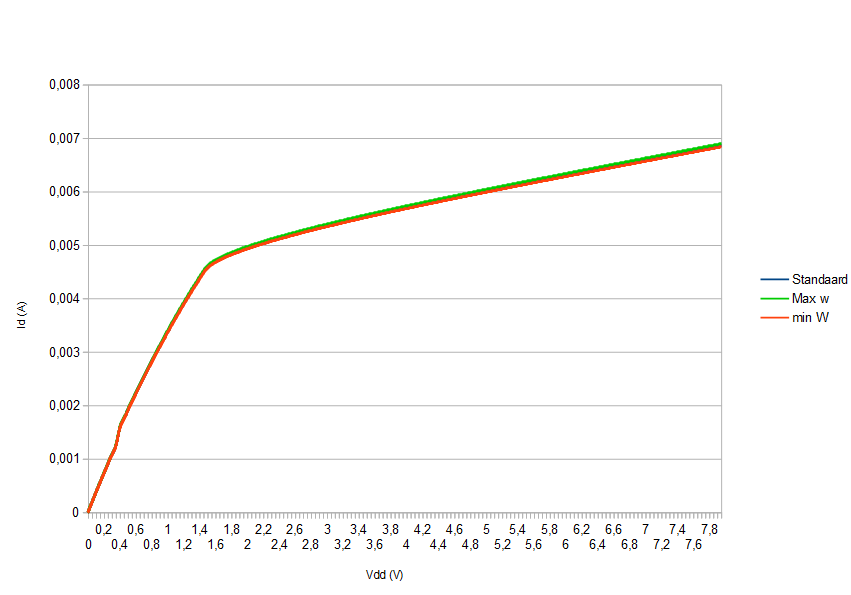
\includegraphics[width=0.8\textwidth]{nmosbreedte}
	\caption{NMOS met de breedte als parameter}
\end{figure}

\begin{figure}[H]
	\centering
	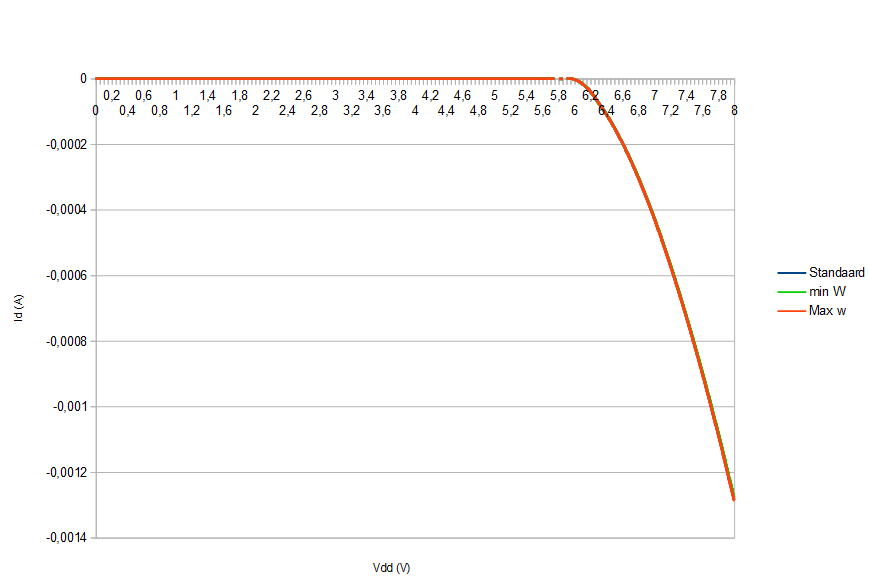
\includegraphics[width=0.8\textwidth]{pmosbreedte}
	\caption{PMOS met de breedte als parameter}
\end{figure}
\clearpage

als laatste hebben we gesimullerd voor de minimale en maximale stroom die door de transistor kan lopen als gevolg van process variaties.

\begin{figure}[H]
	\centering
	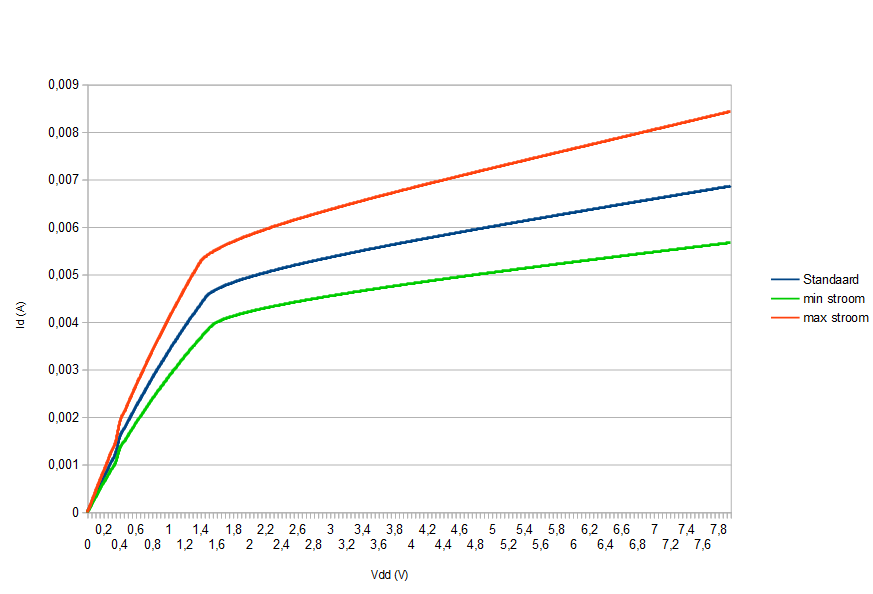
\includegraphics[width=0.8\textwidth]{nmosminmax}
	\caption{De minimale en maximale stroom door de NMOS}
\end{figure}

\begin{figure}[H]
	\centering
	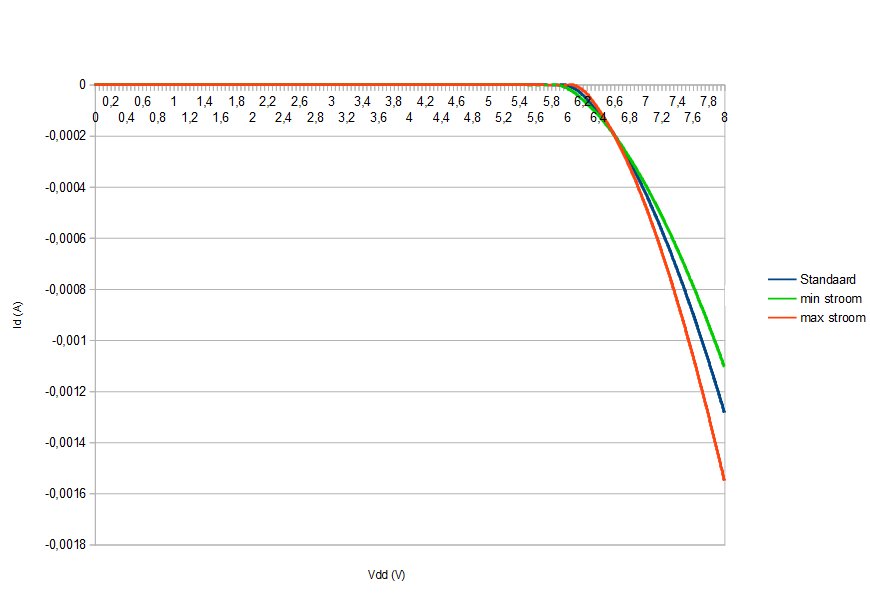
\includegraphics[width=0.8\textwidth]{pmosminmax}
	\caption{De minimale en maximale stroom door de PMOS}
\end{figure}

Hieronder zijn alle resultaten weergegeven in tabellen met de percentages van de afwijking van de normale stroom. Eerst voor de NMOS en daarna voor de PMOS transistor.

\begin{figure}[H]
	\centering
	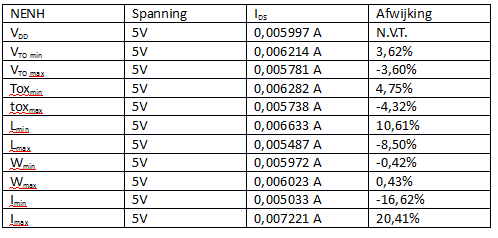
\includegraphics[width=0.8\textwidth]{nenhtabel}
	\caption{Tabel met resultaten voor de NMOS}
\end{figure}

\begin{figure}[H]
	\centering
	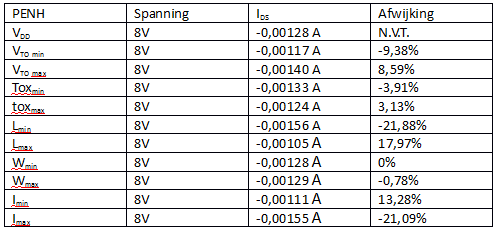
\includegraphics[width=0.8\textwidth]{penhtabel}
	\caption{Tabel met resultaten voor de PMOS}
\end{figure}

\section{Discussie}

Zoals in de theorie is besproken gaven alle veranderingen in de parameters de juiste uitkomst, als je dus de lengte minimaliseerd wordt de stroom door de de transistor groter zoals ook in formule (1) verwacht zou worden. Dit gold dus voor alle parameters die we getest hebben. Wat wel opviel is dat het veranderen van de lengte met 0.1\textmu m veel meer effect op de stroom heeft dan de het veranderen dan de breedte met 0.1\textmu m dit verschil is goed te zien in figuren: 6, 7, 8, 9.\\
In de tabellen zijn de exacte waardes te vinden die de grafieken ondersteunen.\\
Ook valt het op dat alle verandering in de NMOS meer effect hebben op de stroom die er gaat lopen dan de verandereingen in de PMOS, dit komt omdat beide transistoren allebei evengroot zijn genomen en er door een PMOS dan altijd al minder stroom loopt dan door een NMOS en dus in verhouding ook een kleinere verandering zal optreden als een parameter afwijkt van de standaarwaarde.
Met deze resultaten kan er bepaald worden wat de foutmarges mogen zijn bij het produceren van transistoren. En ook waar je rekening mee moet houden tijdens het ontwerpen van een transistor schakeling, dit wil zeggen dat het heel goed kan zijn dat de stroom die er gaat lopen door de transistor niet overeenkomt met wat er misschien verwacht wordt. Dus ook als men een transistor schakeling gaat ontwerpen in een simulatie omgeving zoals PSpice dat er met deze process variaties reken moet worden gehouden voor een betere kans dat de schakeling het ook daadwerkelijk doet als deze eenmaal gefabriceerd is.


\section{Conclusie}

Uit deze resultaten kunnen we dus concluderen dat de resultaten verwacht waren volgens de theorie. Wat nog wel onderzocht zou kunnen worden is bijvoorbeeld het effect van de temperatuur op de transistor of eventueel andere natuursomstandigheden.\\
Verder is er duidelijk te zien welke parameters van een transistor een groter effect hebben op de stroom die er gaat lopen dan andere  dit geeft dus ook aan welke onderdelen van het fabricage process het nauwkeurigst moeten gebeuren zodat de kans op niet goed werkende transistoren te verkleinen.

\section{Bronvermelding}

\begin{itemize}
	\item Jan M. Rabaey, Anantha Chandrakasan, and Borivoje Nikolic (2002), 'Digital Integrated Circuits: A Design Perspective', Hoofdstuk 3 , pagina 120 tot en met pagina 122: 'A word on process variations'.[1]
	\item Nick van der Meijs (2013),\url{http://ens.ewi.tudelft.nl/~nick/courses/gs/slides/01_devices_6up.pdf} , TU Delft course: 'Geïntegreerde schakelingen'.[2]
\end{itemize}
\end{document}
